\section{Problem Statement}

\subsection{Input}

\begin{enumerate}
    \item a directed acyclic graph $\graph = \tuple{\vertices,\edges}$;
    \item a multi-dimensional weight function $\function{\weight}{\vertices}{\weightCodomain}$, where $\wn \in \natural$;
        \subitem We will usually write $\weightE = \apply{\weight}{\solutionE}$
    \item a maximum capacity of the knapsack $\maximumWeight \in \weightCodomain$;
\end{enumerate}

Besides that, one requires the input to satisfy the constraints below \cite{bib:constrained-knapsack}, otherwise the problem would be trivial:

\begin{enumerate}
    \item $\weightE \leqslant \maximumWeight$: the weight of each vertex must be smaller than the knapsack capacity;
    \item $\Sum{\solutionE \in \vertices}{}{\weightE} \geqslant \maximumWeight$: the weight of all vertices combined must be greater than the knapsack capacity;
\end{enumerate}

\subsubsection{Partial Order}

\begin{defn}[Partial Order on Directed Acyclics Graph]
    Given a directed acyclic graph $\graph = \tuple{\vertices,\edges}$, we define the set:
    \begin{equation}
        \partialLower
        \ =
        \SetOf
            {\tuple{\solutionE, \solutionE'}}
            {\mbox{there is a path from the second to the first}}
    \end{equation}
    and so $\partialLower$ is a partial order over the set $\vertices$.
\end{defn}

\begin{figure}[ht!]
    \centering
    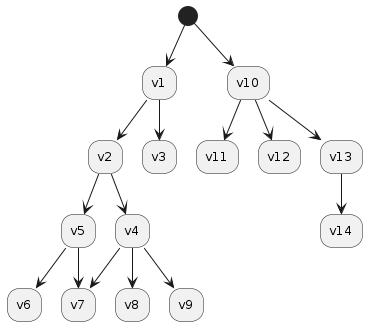
\includegraphics[width=0.5\textwidth]{images/directed acyclic graph.png}
    \caption{Example of a directed acyclic graph. The black dot indicates the root vertices. For this case, the induced partial order satisfy: $v5 \partialLower v2$, $v7 \partialLower v1$, $v14 \partialLower v10$.}
\end{figure}

\subsection{Output}

A subset $\solution \subseteq \vertices$ of the vertices which satisfy:

\begin{equation}
    \label{eq:capacity-constraint}
    \Sum
        {\solutionE \in \solution}
        {}
        {\weightE}
    \leqslant
    \maximumWeight
\end{equation}

\begin{equation}
    \label{eq:precedence-constraint}
    \forAll
        {\solutionE}
        {\ifThen
            {\solutionE \in \solution}
            {\forAll
                {\solutionEp}
                {\ifThen
                    {\solutionE \partialLower \solutionEp}
                    {\solutionEp \in \solution}
                }
            }
        }
\end{equation}

\eqref{eq:capacity-constraint} states the total weight of all vertices in the solution set $\solution$ must not be greater than the weight limit $\maximumWeight$. It is called \capacityConstraint.

\eqref{eq:precedence-constraint}\footnote{It is a First-order logic expression \cite{bib:logic}.} says that, if a $\solutionE$ is included in the solution, then all the $\solutionEp$ greater than it (in the sense of the partial order $\partialLower$) must also be included. It is called \precedenceConstraint.

\subsection{Objective}

Find $\solution$ that maximizes $\abs{\solution}$. In other words: find the solution with the maximum number of vertices.
